\begin{comment}
  What is the original framing of the problem? It almost doesn't make sense to frame it as a system-wide problem. Because a process is useless if it's totally isolated from the rest of the system. Make processes isolated and poke some holes in this isolation.

  This is something that has been on the radar since the origin of multi-processing
  systems.  We can argue that one of the reasons it's never been solved has been because
  the problem is too broadly defined.

  One set of tehcnologies that has helped in this sense has been hypervisor-based
  virtualization. But this is subject to some fundamental concerns. Containers

  It's a reframing but it's also narrowing the scope
  A "scoping definition"? A "scoping reframing"?
  Applying it specifically to containers and virtualization
\end{comment}


Researchers have been studying confinement for decades~\cite{lampson1973_confinement}, and
have been designing and applying confinement primitives since the early days of
time-sharing computers and multi-tenant systems~\cite{shu2016_security_isolation_study}.
While many developments have been made in the mean time, the current confinement landscape
(particularly within the Linux ecosystem) suffers from a few fundamental flaws that
culminate in poor container security practices; this does not need to be so. This chapter
presents a critique of the current state of confinement on Linux, examines how confinement
primitives are applied to containers, and proposes a fundamental re-framing of the problem
to focus on complexity, adoptability, and suitability for container-specific applications.
In light of this re-framing, we consider design goals for \bpfbox{} and \bpfcontain{} and
present the threat model for confinement under these research systems.

\section{Rethinking the Virtualization Narrative}%
\label{s:cp-rethinking}

\todo{Have a diagram that positions virtual machines, containers, and standalone in terms
of perceived isolation guarantees, have an arrow spanning left to right. We are trying to
move containers as far to the right as possible, ideally to the same place as
hypervisor-based virtual machines, hopefully farther over. On the right: isolation
provided by hardware, isolation provided by software (perceived stronger vs perceived
weaker). When the boundary is in hardware it is considered rigid, in software things are
considered more malleable. We are trying to find a way to make things more rigid in
software.}

Hypervisor-backed virtualization is commonly considered more secure than
con\-tain\-er-based virtualization~\cite{sultan2019_container_security,
eder2016_hypervisor_container}.  \todo{See figure ...} Intuitively, this makes sense.
Containers run directly on the host operating system, whereas a virtual machine runs on
top of a hypervisor, separated by at least one layer of indirection from the host system.
However, this intuition does not strictly stand up to scrutiny. A virtual machine running
on top of a hypervisor makes requests to the hypervisor's \gls{api} (via hypercalls), in
much the same way as a container running on a host operating system makes requests to the
kernel's \gls{api} (via system calls).  \Cref{fig:syscall-hypercall} illustrates this
parity.

\begin{figure}[htbp]
  \centering
  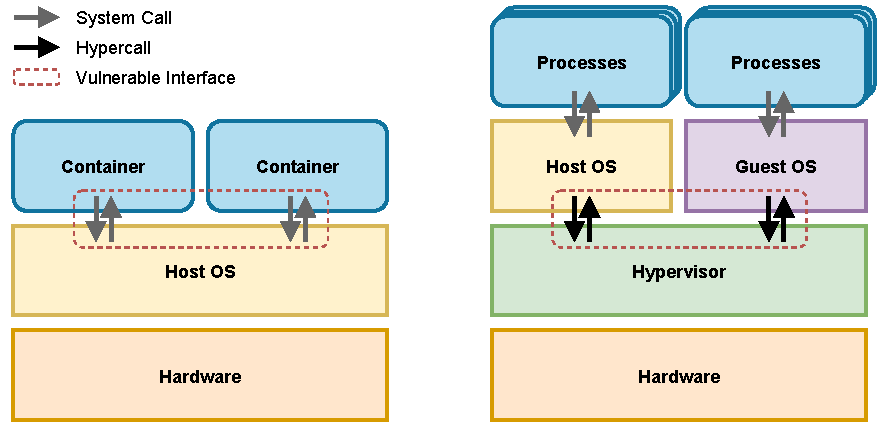
\includegraphics[width=0.8\linewidth]{figs/confinement-problem/syscall-hypercall.pdf}
  \caption[System calls and hypercalls as vulnerable interfaces]{
    System calls and hypercalls as vulnerable interfaces. Containers (which are really
    just process groups running on the host \gls{os}) make system calls to the
    more-privileged host \gls{os} kernel. Similarly, a guest operating system makes
    hypercalls to the more-privileged hypervisor. Both of these interfaces are ripe
    targets for a myriad of attacks, including privilege escalation and tampering with
    sensitive resources. This parity becomes particularly evident when we assume that an
    attacker has or is able to obtain control over the guest \gls{os}.
  }%
  \label{fig:syscall-hypercall}
\end{figure}

\todo{You can't craft fine-grained policies with a virtual machine. You get a box. Network
firewalls, shared filesystem with access controls. (The cognitive overhead to lock down
a virtual machine after exposing specific interfaces is very high.) With a virtual machine,
policy is intrinsically tied to functionality. It's all about configuring the interfaces
and then locking it down (either from the inside or outside). Provision the resource and
secure it, because that's how you do it with a conventional operating system. Here, the
provisioning is already taken care of by the operating system, so all we're doing is
specifying the access.}

\todo{Verify the following: VM escapes are partially about exploiting bugs, but it's also
that the attacker has access to a lot of functionality that allows them the opportunity to
exploit these bugs. It's not least-privilege. You're giving them an entire VM. They have
control over the entire OS and the entire hardware interface becomes an attack surface. In
principle, with a container, you can make this exposed interface very small. People think
of the hardware interface as being more secure, even though in principle it is larger,
since it is rigid. But we have a hard boundary in the Linux kernel too: the \gls{lsm}
layer. People think of hardware as being more secure, and somehow they think this notion
carries forward to hardware semantics implemented in software.}

\todo{We have a repeated mistake here: Taking the interface that's there as the one we use
to define our security properties. When we build containers, we made the mistake again of
thinking that the interfaces are rigid, and that we need to make use of the abstractions
that already exist. For the people who are designing container runtimes, their goal is to
design container runtimes, not reinvent security mechanisms. Our goal is not to design
a new container runtime, it's to improve the security of existing runtimes.}

% The isolation guarantees provided by a virtual machine come almost entirely from a sense
% of obfuscation over a semantic gap, created as the hypervisor virtualizes system
% resources. There is no notion of centralized policy in a virtual machine; rather, security
% is an emergent phenomenon, a form of \enquote{policy through mechanism}. With the right
% tools, we can and have poked holes everywhere in this
% policy~\cite{dubrelle2015_hypervisor, thongthua2016_analysis, shahzad2017_systematic}.

The central argument of this thesis is that there is no fundamental reason why containers
cannot be as\,---\,if not more\,---\,secure than virtual machines. While it is true that
a containerized process is nothing more than a host process running under some virtualized
state, an operating system that provides and enforces the right set of confinement
primitives should be able to lock a container down in much the same way that a hypervisor
implicitly enforces isolation. \todo{Talk about why containers suck in brief and lead into 3.2}

\todo{All of the following should be moved into another section, possibly design goals,
possibly something else?}

\todo{Introduce \bpfbox{} and \bpfcontain{}}

Unlike hypervisor-based isolation, a policy enforced by the operating system has the
potential to be more minimal, centralized, and accessible to end-users. The key to
developing such an enforcement mechanism lies in defining a clear protection boundary
within the kernel and enforcing access across this boundary. \bpfbox{} lays the foundation
for such an enforcement mechanism, and \bpfcontain{} explicitly applies it to containers.

\todo{Rephrase this: Our goal is to have policies that are centralized, flexible, ...}
In \bpfbox{}, policies are defined in a centralized, flexible policy file. Using
\gls{ebpf}, \bpfbox{} can observe various aspects of system behaviour, such as user and
kernelspace function calls, and incorporate them into its enforcement decisions. This
helps define fine-grained policy while keeping the overall policy syntax clean and simple.
\bpfcontain{} extends this model by defining an implicit protection boundary around
a container, where the container is made up of a set of host processes and associated
resources. Operations \textit{within} the container are implicitly allowed, whereas
operations \textit{outside} the container or operations that can affect the system as
a whole are implicitly denied. In this way, \bpfcontain{} policy allows the user to define
\textit{exceptions to implicit rules} rather than the rules themselves.

The key insight behind both \bpfbox{} and \bpfcontain{} is that novel kernel mechanisms
are required to realize their respective goals. The new \gls{ebpf} kernel technology
provides precisely the right framework for developing such mechanisms. In \bpfcontain{},
a clear and well-defined abstraction for containers allows the kernel to enforce implicit
policy centred around container semantics. We rely on \gls{ebpf} to enable the definition
of such an abstraction without necessarily tying the kernel down to one specific
interpretation of what a container actually is. Using multiple \gls{ebpf} programs and
maps, we can combine various other aspects of system behaviour with \gls{lsm}-based
enforcement in a stateful manner. \bpfbox{} uses its ability to introspect system state to
enable policy enforcement at the granularity of individual function calls.

At this point, it should be clear that both \bpfbox{} and \bpfcontain{} leverage the power
of \gls{ebpf} to make improvements on the existing status quo of Linux confinement. The
next two sections, \Cref{s:cp-issues} and \Cref{s:cp-containers}, discuss the state of
confinement on Linux and how existing container technologies apply confinement primitives.
This discussion serves to contextualize the notions behind this section and motivates the
need for \bpfbox{} and \bpfcontain{} as novel confinement primitives.

% \begin{inprogress}
%   \begin{itemize}
%     \item Just like the word container makes people think about security
%     \item Type I and Type II hypervisor, the way it's depicted, makes people think something else is happening
%     \item The representation and terminology
%     \item This makes sense to talk about it if we connect it to containers
%     \item Why can't containers give as good or better security than hypervisors
%     \item Can we just get our enforcement clear
%     \item Virtual machines seem like they define a clear boundary, but it isn't actually
%           so clear in practice because all these things are being shared across boundaries
%     \item People think of virtual machines as being inherently more secure, the security
%           benefit is more of an obfuscation thing related to the semantic gap but with the right
%           tools you can still cross it freely
%     \item VMs have all these little holes everywhere and the policy is not centralized\,---\,we
%           have policy through mechanism
%     \item There's no reason why containers can't be as (if not more) secure than virtual machines
%     \item Because we can make this boundary very clear
%     \item \bpfcontain{} can be seen as a step towards this
%   \end{itemize}
% \end{inprogress}



\section{Fundamental Issues with Linux Confinement}%
\label{s:cp-issues}

Here we identify three fundamental issues with the current state of Linux confinement and
contextualize them with examples from existing container and confinement frameworks. This
section serves to provide a framing of an additional context for the container-specific
issues, discussed in \Cref{s:cp-containers}, and the design goals for \bpfbox{} and
\bpfcontain{}, discussed in \Cref{s:cp-design}.


\begin{enumerate}[font=\bfseries]
  \item \textbf{Complexity, Interdependence, and Inflexibility.}
    Existing confinement primitives are overly complex and designed for use cases beyond
    simple process confinement. To achieve simple confinement, frameworks must abuse and
    recombine a number of existing primitives, each designed for a different use case.
    Namespaces~\cite{biederman2006_namespaces, linux_namespaces} were designed to
    virtualize resources; they do not provide confinement by themselves. To truly confine
    a process using namespaces, we need a way to account for namespace escapes.
    Cgroups~\cite{cgroups}, similarly, were designed to virtualize the availability of
    quantifiable resources, not to directly confine. Unix
    \gls{dac}~\cite{jaeger2008_os_security, van_oorschot2020_tools_jewels} is far too
    coarse-grained and easy to bypass to be directly useful for confinement. POSIX
    capabilities~\cite{posix_capabilities} can be used to reduce overprivilege by
    partitioning root privileges, but these do not implement confinement by themselves.

    Seccomp-bpf~\cite{seccomp, edge2015_seccomp} works well to reduce the attack surface
    exposed by system calls, but writing classic \gls{bpf} filters is a complex and
    error-prone process. Fine-grained filtering quickly becomes untenable, particularly
    when considering race conditions when checking system call arguments and system call
    equivalence classes.  Linux \gls{mac} can be used to implement true confinement, but
    a typical \gls{lsm} like AppArmor~\cite{cowan2000_apparmor} or
    SELinux~\cite{smalley2001_selinux} is designed for use cases beyond simple sandboxing.
    These mechanisms are designed to implement and enforce system-wide \gls{mac} policy,
    not simple process-level confinement~\cite{belair2019_leveraging}. Further, major
    \glspl{lsm} are statically loaded and unstackable, meaning that end-users must
    generally choose one major solution with little room to adjust enforcement at runtime.

    To implement confinement, sandboxing and containerization frameworks generally mix and
    match the aforementioned solutions\,---\,some of which were designed for confinement,
    some of which were not, and none of which were designed for \textit{simple,
    process-level} confinement. LXC, Docker, Snap, and others all combine namespaces,
    cgroups, capabilities, seccomp-bpf, and AppArmor/SELinux policy to achieve
    confinement. In the case of Snap, high-level abstractions in policy definition can
    simplify the process of policy authorship to a certain extent, but simple policies
    are still compiled down into thousands of lines of policy soup, spanning multiple
    confinement mechanisms.

  \item \textbf{Unsuitability for Containers.}
    Existing Linux \gls{dac} and \gls{mac} is unsuitable for containers.
    \gls{lsm}-based \gls{mac} implementations like AppArmor and SELinux are
    designed to implement global, system-wide confinement policy; they are not designed
    for ad-hoc, process-level confinement~\cite{belair2019_leveraging}. Additionally,
    these \gls{lsm} implementations were not designed with containers in mind and thus
    do not consider container semantics in policy definition and enforcement. This lack
    of semantic awareness further complicates policy authorship for containers and
    forces the end-user to make compromises between security and functionality.

    Sultan \etal~\cite{sultan2019_container_security} suggest that the container
    security community should move towards a container-specific \gls{lsm}
    implementation. Security namespaces, proposed by Sun
    \etal~\cite{sun2018_security_namespace} can be seen as a partial step toward solving
    this problem.  Under security namespaces, each container can load and use its own
    \gls{lsm} of choice, but these \glspl{lsm} would still be subject to many of the
    same aforementioned restrictions. That is, existing \glspl{lsm} are not designed
    with container semantics in mind. A truly container-specific \gls{lsm} could incorporate
    container semantics into policy enforcement for cleaner and more effective policies.

    \gls{uid} remapping under a new user namespace does help with the \gls{dac} case by
    remapping root to a non-root \gls{uid}, but this is only really helpful for limiting
    the power of root. Other limitations of \gls{dac} still apply. For instance,
    a world-readable file could still be used for information disclosure or
    a world-writable file could still be the target of data corruption. For such reasons,
    \gls{dac} alone appears to be fundamentally insufficient for true isolation between
    host and container. Thus, to achieve proper process-level confinement for containers,
    we need an \gls{lsm}-based solution that is aware of container semantics.

  \item \textbf{Difficulty Adopting New Solutions.}
    Motivated by the inherent difficulties associated with the existing confinement space,
    academics are often tempted to propose new confinement solutions. Many try to solve
    the problem by simply recombining and reusing existing primitives in new and
    innovative ways.  However, these types of solutions generally are not really a step
    forward with respect to addressing the issues in items 1 and 2, since these are
    emergent properties inherent to the underlying confinement primitives themselves.

    In order to truly solve these fundamental issues, we need kernel support for new
    primitives. Unfortunately, this begets yet another fundamental issue: adding new
    solutions directly to the kernel is difficult, particularly from an adoptability
    standpoint. New kernel code can introduce bugs and security vulnerabilities, and needs
    to be throughly tested before it can be considered production ready. Paradoxically,
    the potential to introduce new security vulnerabilities can make the use of such novel
    primitives \textit{less} secure. Similarly, kernel bugs can introduce availability
    concerns in production systems, even when such bugs are not security-critical. For
    these reasons, industry managers may be reluctant to adopt new, out-of-tree solutions
    based on loadable kernel modules, for example~\cite{gregg2019_bpf}.

    Another adoptability concern arises when we consider \textit{container-specific}
    confinement~\cite{sultan2019_container_security, sun2018_security_namespace} as an
    end-goal.  To date, the definition of precisely what a container is has been more or
    less in flux. The requirements and precise specifications of what constitutes
    a container tend to change as container frameworks evolve and new use cases crop up.
    If not everyone can agree on what a container even is, how can we expect to reach
    agreement on which underlying container security abstraction should be merged into the
    mainline kernel? To solve this problem, we need a way to add abstractions into the
    kernel in such a way that is neither binding nor limited by the lack of adoptability
    associated with traditional kernel-based solutions. These requirements motivate the
    use of \gls{ebpf} for designing a container-specific security solution, and thus
    motivate the design of \bpfbox{} and \bpfcontain{}.
\end{enumerate}



\section{How Containers Apply Confinement Primitives}%
\label{s:cp-containers}

This section examines and critiques the way Linux container technologies apply confinement
primitives to lock down container deployments. We focus primarily on Docker as a case
study, however these principles in general apply to the majority of container management
frameworks.

In general, Linux containers have three broad goals. However, these goals are neither
equally met nor equally prioritized by existing container management frameworks. In order
of decreasing prioritization, they are:
\begin{enumerate}[font=\bfseries]
  \item \textbf{Dependency Management / Reproducibility.}
    Containers should provide an easy and robust framework for creating reproducible
    development environments. Dependencies should be maximally self-contained such that
    a containerized environment \enquote{just works} to the maximum possible extent. We
    can see examples of this property in Docker, the predominant container framework to
    date. Docker Hub~\cite{docker_hub} allows container images to be pulled from the
    Internet, recombined, and used to create further images. The end result is a flexible
    framework for creating and distributing reproducible development environments.

  \item \textbf{Virtualization.}
    Containers should virtualize system resources, creating the illusion of running on
    a separate physical machine. Where possible, resources should be transparently reused
    between multiple containers (e.g.~sharing a single base copy of the same shared
    library between two container images).

    To achieve virtualization, containers generally rely on the namespaces and cgroups
    primitives provided by the Linux kernel.  Overlay filesystems~\cite{overlayfs}
    combined with the mount namespace allow containers to perform one-way sharing of
    filesystem resources. The PID namespace allows each container to have its own
    \textit{init} process and virtual process tree.  The network namespace allows the
    container to virtualize its network devices while the UTS namespace virtualizes host
    and domain names. Process control groups virtualize other resources such as the CPU,
    main memory, and device drivers.

  \item \textbf{Confinement.}
    Containerized processes should be confined by default. That is, a containerized
    process should have access to the minimal set of privileges required for it to operate
    normally. The extent to which this property is achieved by conventional container
    frameworks varies greatly, both by framework and by individual
    deployment~\cite{sultan2019_container_security, lin2018_container_security,
    bui2015_docker_analysis}. In general, proper confinement is not a priority of
    container frameworks, and this tends to result in sacrificing security for
    ease-of-deployment.
\end{enumerate}

The aforementioned goals are not only ordered by their decreasing prioritization in extant
container management frameworks; they are also ordered by increasing relevance to
container security. That is to say, existing frameworks generally prioritize goals
unrelated to security and leave security as an afterthought. Since containers are really
just process groups running directly on the host operating system, an unconfined container
therefore exposes the same attack surface as an ordinary host process. Thus, one might
expect container security to be of paramount importance. Unfortunately, this is not the
case. These difficulties in confinement motivate the need to revisit container security
and approach it from a confinement-first perspective. To understand how these confinement
issues impact containers, we briefly review how container management systems apply
confinement primitives in practice.

To achieve confinement in the first place, container frameworks cobble together existing
confinement technologies and apply them ways that are often simultaneously confusing and
difficult to audit. The result is a complex policy soup with little room for customization
or auditability. For instance, Snap~\cite{snap} uses a high-level policy language that
targets system interfaces in a coarse-grained manner. Under the hood, this is compiled
into hundreds or thousands of lines of seccomp-bpf and AppArmor policy.
Docker~\cite{docker_security, docker_default_apparmor, docker_apparmor} uses a generic
AppArmor, seccomp-bpf, and POSIX capability policy for every container, along with default
namespace and control group configurations. Making meaningful changes to these policy
configurations, beyond simply disabling them altogether, is difficult and
error-prone~\cite{lin2018_container_security}.

Container security policies are often overly-generic and ill-suited to fine-grained
confinement. Part of the problem here is that containers in general are designed to
\enquote{just work}. Overly fine-grained security policies may get in the way of this,
particularly as end-user requirements vary and evolve across deployments.
Docker~\cite{docker_security}, for instance, provisions an overly-permissive default
AppArmor policy~\cite{docker_default_apparmor} designed to enforce basic protections
against interacting with sensitive kernel parameters without impacting the functionality
of the container. \todo{More examples}

Even worse, many container management systems operate under a fail-open approach when the
necessary security mechanisms are not supported. This results in low-security deployments,
often without even notifying the user that there may be such a configuration. Since the
end-user generally doesn't even participate in the policy authorship process, they may not
even be aware of the level of protection that is being applied, resulting in a dangerous
false sense of security. Docker's AppArmor policy~\cite{docker_apparmor,
docker_default_apparmor}, for instance, is not applied when the deployment environment
doesn't support AppArmor or AppArmor is disabled. Snap~\cite{snap} and others that rely on
the AppArmor or SELinux \glspl{lsm} for confinement suffer from similar failings.

Other aspects of confinement policy may be ignored entirely or even worse, overridden by
a more permissive policy, possibly without the user's knowledge.
Docker~\cite{docker_security} applies a dangerously permissive iptables policy that can
transparently expose a container to an external network, even overriding existing deny
rules. This overly-permissive network policy was the direct cause of a recent data breach
at NewsBlur~\cite{newsblur}, a news aggregation website, although NewsBlur administrators
claim that no user data was actually compromised~\cite{newsblur}. \todo{More examples}



\section{Design Goals}%
\label{s:cp-design}

Using the above analysis of the confinement problem, we can derive a clear set of design
goals for \bpfbox{} and \bpfcontain{}, such that they approach a solution to issues that
plague the status quo. In particular, we derive the following three design principles.
Note that these design principles are each the polar opposite of the three major problems
identified in \Cref{s:cp-issues}.

\begin{enumerate}[font=\bfseries]
  \item \textbf{Simple, Self-Contained, and Flexible.}
    \bpfbox{} and \bpfcontain{} should be simple, self-contained, and flexible.  The
    policy language for each should be as simple as possible without sacrificing
    expressiveness, and should not rely on any manual labelling of system resources as in
    SELinux~\cite{smalley2001_selinux}. \bpfbox{} and \bpfcontain{} should be able to
    fully confine a process without the relying on additional confinement primitives; that
    is, the enforcement engines underlying \bpfbox{} and \bpfcontain{} should be fully
    self-sufficient.

    The policy language for \bpfbox{} and \bpfcontain{} should be as flexible as possible,
    supporting multiple distinct use cases from basic sandboxing, to addressing specific
    vulnerabilities in an application, to full-fledged container deployments. Using
    \gls{ebpf}, \bpfbox{} and \bpfcontain{} can incorporate additional system state into
    enforcement decision, beyond the state exposed by \gls{lsm} hooks. The ultimate goal
    of \bpfbox{} and \bpfcontain{} is to make fine-grained confinement accessible to the
    end-user, without the need to rely on complex configuration, unnecessary setup, or the
    combination of multiple confinement primitives.

  \item \textbf{Process- and Container-Specific.}
    \bpfbox{} and \bpfcontain{} should process- and container-specific respectively by
    design. In particular, this means that \bpfbox{} should be designed with process-level
    confinement in mind and \bpfcontain{} should enforce policy in such a way that it is
    aware of container-level semantics such as namespace and cgroup membership.

  \item \textbf{Adoptable.}
    Both \bpfbox{} and \bpfcontain{} should be readily adoptable in production
    environments, the cloud, and even personal desktop environments. In particular, the
    requirements to run these mechanisms should be minimal, all privileged code should be
    safe to use in production, system overhead should be in line with existing confinement
    mechanisms, and both \bpfbox{} and \bpfcontain{} should work out of the box on an
    unmodified, vanilla version of the Linux kernel. To support these goals, \bpfbox{} and
    \bpfcontain{} leverage the adoptability guarantees provided by \gls{ebpf} along with
    a modular design that focuses on simplicity. For additional security, \bpfbox{} and
    \bpfcontain{} support confinement without requiring setuid root binaries and all ring
    0 code passes through the \gls{ebpf} verifier before it is loaded into the system.
\end{enumerate}





\section{The \bpfbox{} and \bpfcontain{} Threat Model}%
\label{s:cp-threat-model}

This section outlines the threat model for \bpfbox{} and \bpfcontain{}. In particular, we
provide a scoping definition of confinement policy and what it means for a policy
enforcement mechanism to confine a subject using that policy. We also discuss the
adversary's capabilities, goals, and potential attack vectors in a commodity Linux-based
operating system. In general, both \bpfbox{} and \bpfcontain{} have a very similar threat
model, with subtle and specific differences arising in a few key areas. Where
discrepancies arise, they will be noted accordingly.

\subsection{Confinement Policy and Enforcement Engine}

We define \textit{confinement} as the restriction of \textit{subject} (system actors such
as processes) behaviours to a set of desired behaviours, as they pertain to
\textit{objects} (system resources such as files, network sockets, devices, and IPC
handles onto other subjects). Consider the set of all subjects $\mathcal{S}$ and the set
of all objects $\mathcal{O}$. We define $\mathcal{S} \subseteq \mathcal{O}$ to account for
IPC objects. The goal is to create a confinement policy $\mathcal{P}_i$ for a subject
$\mathcal{S}_i$ that maps $(\mathcal{S}_i, \mathcal{O}_j, Op)$ tuples to \textit{policy
decisions} where $Op$ is an operation $\mathcal{S}_i \xrightarrow{Op} \mathcal{O}_j$.  The
policy is written in some abstract policy language that encodes such tuples in
a human-readable format.

An \textit{enforcement engine} operates between the subject and system objects. It
intercepts requests to access these objects and makes an access control decision according
to the corresponding confinement policy. The end result is a behavioural restriction on
the subject to some subset of all possible behaviours. The goal of an effective
confinement policy and enforcement engine is to achieve the minimal possible subset for
normal operation, thus achieving the principle of least privilege and minimizing the
attack surface for potential exploitation.

Under \bpfbox{}, the enforcement engine targets access at the process level, interposing
on individual system calls using \gls{ebpf} programs attached to \gls{lsm} hooks and
enforcing access based on per-executable policies. Under \bpfcontain{}, this enforcement
is expanded to operate at the container level. Like \bpfbox{}, \bpfcontain{} interposes on
system calls using \gls{ebpf} programs attached to \gls{lsm} hooks, but these programs
account for the state of an individual container, including properties like a process'
container membership and whether a given resource is part of a container-local namespace.
In effect, this means that, unlike \bpfbox{}, \bpfcontain{} defines a clear protection
boundary around the container itself; access to resources \textit{within} the container is
considered default-allow, whereas resources \textit{outside}  of the container or
operations that can affect global system state are considered default-deny.

% When designing a policy language and policy enforcement engine, there are a few trade-offs
% to consider that can directly impact the security, usability, readability, and
% auditability of resulting policies. We discuss them as follows.

% \paragraph*{Expressive vs Terse} An \textit{expressive} confinement policy encodes rules
% (our subject, object, and operation tuples) at a fine granularity. Conversely,
% a \textit{terse} confinement policy encodes rules at a coarse granularity. A more
% expressive policy language is naturally conducive to the principle of least-privilege, as
% fine-grained access controls can tightly confine an application to the minimal set of
% desired behaviours.  Intuitively, a terser policy language is less conducive to
% a least-privilege confinement policy, as it becomes impossible to encode access controls
% at the required granularity. However, policy authorship becomes significantly easier under
% a terse policy language~\cite{schreuders2012_towards}. This property may indirectly
% improve security in practice, as users are less likely to take shortcuts during policy
% authorship.

% \paragraph*{Restrictive vs Permissive} A more \textit{restrictive} policy language
% takes a
% \begin{inprogress}
%   \begin{itemize}
%     \item Here, restrictive and permissive refer to the implicit policy action when
%           a particular policy rule is left undefined
%     \item Due to the high complexity of systems, it rapidly becomes untenable to write an
%           individual policy rule for each aspect of the system, particularly in
%           highly-expressive policy languages
%     \item Thus, some default action is required when \todo{Finish}
%     \item Restrictive policy languages take a deny-first approach to
%   \end{itemize}
% \end{inprogress}

\subsection{The Adversary and Attack Vectors}

We consider a privileged remote adversary with root-level access under conventional Unix
discretionary access controls.  Further, as assume that the adversary has already achieved
local code execution at the process level. This means that the adversary is capable of
running arbitrary code in the context of a given process or container and can perform
arbitrary interactions with the kernel's reference monitor; these interactions may be
allowed or denied at the discretion of the reference monitor, and may or may not result in
the subsequent execution of kernel code, such as system call implementations. Without any
confinement in place, the adversary is capable of reading or writing any file, accessing
any device, loading kernel code, and performing any other privileged operation.

Our goal is to confine the adversary such that they are unable to access
security-sensitive resources, interfere with external processes, make changes to global
system state, or perform any other operation in violation of our security model.  The
adversary's goal is simple: to escape confinement. This goal of escaping confinement
(tantamount to privilege escalation) can be a subgoal used to achieve some other purpose,
such as spoofing, tampering, information disclosure, or persistence.



\section{Summary}

This chapter has presented a novel framing of the confinement problem as it pertains to
Linux and Linux containers. In particular, we reexamine the differences between virtual
machines and containers and argue that the former need not be more secure than the latter,
we identify three distinct problems with modern Linux confinement, and we examine how
containers apply existing confinement primitives. This re-framing of the confinement
problem both serves as a motivation for the creation of \bpfbox{} and \bpfcontain{} and
informs the design goals behind these two research systems. Finally, we present
a high-level threat model for \bpfbox{} and \bpfcontain{}, providing a scoping definition
for what it means to confine an adversary. The next two chapters, \Cref{c:bpfbox} and
\Cref{c:bpfcontain}, present the design and implementation of \bpfbox{} an \bpfcontain{} in
detail.
